\begin{figure}
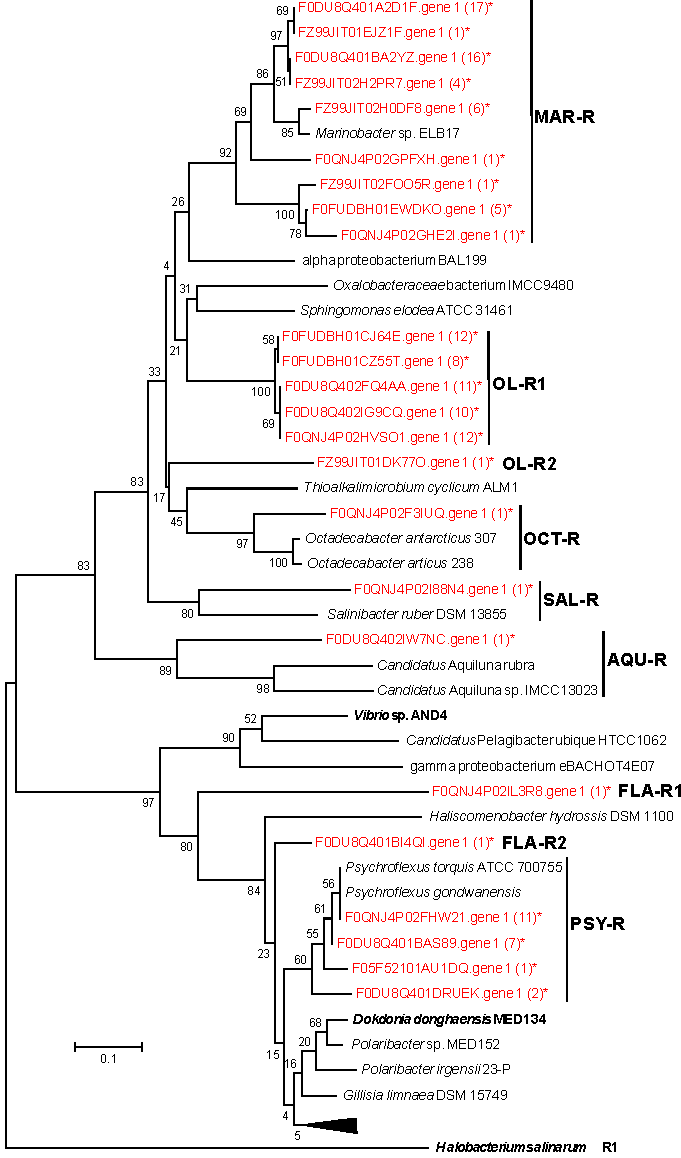
\includegraphics[width=\textwidth]{orglake_figures/rhodopsin_tree.pdf}
\caption[Phylogenetic tree of rhodopsin homologues]{Phylogenetic tree of rhodopsin homologs. \emph{Halobacterium salinarium} R1 halorhodopsin was used as an outgroup. The tree was computed from a 78 amino acid region spanning the motif involved in `spectral tuning' using the neighbour-joining algorithm. Organic Lake sequences from this study are shown in red and marked with an asterisk (*). Numbers in parentheses are counts of sequences that clustered with the Organic Lake homologue shown in the tree with 90\% amino acid identity. Sequences with confirmed activity are shown in bold. Accession numbers from top to bottom are: EAZ99241, EDP63929, EGF32634, ZP\_09955974, AEG32267, EDY76405, EDY88259, YP\_445623, ACN42850, EIC91904, ZP\_02194911, AAZ21446, AAT38609, AEE49633, EAS71907, sequence from John Bowman (personal correspondence), EAQ40507, EAQ40925, EAR12394, EHQ04368 and YP\_001689404.}
\label{fig:rhodopsin_tree}

\end{figure}
